\documentclass[a4paper]{article}
\usepackage[margin=25mm]{geometry}
\usepackage{amsmath}
\usepackage{amsfonts}
\usepackage{amssymb}
\usepackage{graphicx}
\usepackage{verbatim}
\pagenumbering{arabic}
\graphicspath{ {./plots/} }


% Keywords command
\providecommand{\keywords}[1]
{
  \small
  \textbf{\textit{Keywords---}} #1
}

% \tableofcontents

\title{Numerical Solution of Point Defect Equations by MOOSE}
\author{Abdurrahman Ozturk$^{1}$, Karim Ahmed$^{1}$  \\
        \small $^{1}$Texas A\&M University \\
        % \small $^{2}$University B \\
}
% \date{} % Comment this line to show today's date
\begin{document}
\maketitle

\begin{abstract}

We present a detailed investigation of the effect of size on the segregation of point defects to interfaces and the resultant nucleation of voids. We utilize the spatially-resolved rate-theory (SRRT) modeling technique valid for modeling surfaces as discrete sinks. The effects of defect production rate, bias, and profile are thoroughly studied. The model predictions are generally different from the textbook ones obtained by the classical homogenized rate theory approach. The simulations show a strong dependence of the steady state defect profiles on the grain size, temperature, and production rate, bias, and profile. Moreover, the sink strength of each boundary is also affected by these factors. Furthermore, it is predicted that whenever there is a production bias, no neutral sinks can exist, i.e., there is always a preference for surfaces/interfaces to absorb one type of defects over another. The model predictions demonstrate the shortcomings of the classical homogenous rate-theory approach and shed light on the limitations of using ion irradiation to mimic neutron irradiation.

% Irradiation of a material creates point defects, vacancies and interstitials, as a result of
% atomic collisions. Those point defects are mobile and able to diffuse through material, recombine with each other,
% and disappear when they react with sinks. The concentration of both vacancy and interstitial can be described mathematically by chemical rate balance equations, named point defect equations (rate theory equations). Production, recombination, diffusion and reaction of point defects are given by separate terms in those equations, which makes it easy to solve and analyze each of them individually. In this work, spatially resolved non-dimensional point defect equations are solved in 1D by using MOOSE Framework. The effect of irradiation dose rate, sink density, temperature, uniform defect production, non-uniform defect production and biased defect production on steady state defect concentration profile and on grain boundary sink strength are studied. The calculations are also repeated for different domain sizes changing from 5\emph{nm} to 5$\mu$\emph{m} to investigate the effect of grain size on defect concentration and grain boundary sink strength. According to results, the domain size and defect production profile/bias have a significant effect on concentration profiles. They could create a flipped concentration profile through domain, which ends up with a defect segregation near grain boundary.

\end{abstract} \hspace{10pt}

%TC:ignore
\keywords{point defect equations, rate theory, interstitial, vacancy, radiation damage, MOOSE}
%TC:endignore

% Word count
% \verbatiminput{\jobname.wordcount.tex}

% \listoftables
% \listoffigures

\section{Introduction} \hspace{10pt}

\section{Methodology} \hspace{10pt}

\begin{table}[h!]
  \centering
  \caption{Material Properties for Nickel\cite{walgraef1996}}
  \label{table:Ni_material_properties}
  \begin{tabular}{ ||p{2cm}|p{2cm}||  }
     % \hline
     % \multicolumn{5}{|c|}{Material Properties} \\
     \hline
     Property & Value\\
     \hline\hline
     a  & 0.352 nm\\
     V  & 0.01206 nm^3\\
     E_{m,i}  & 0.30 eV\\
     E_{m,v}  & 1.30 eV\\
     E_{f,i}  & 4.27 eV\\
     E_{f,v}  & 1.60 eV\\
     D_{0,i}  & 1e-7 m^2/s\\
     D_{0,v}  & 6e-5 m^2/s\\

     \hline
  \end{tabular}
\end{table}

\begin{table}[h!]
  \centering
  \caption{Simulation Parameters}
  \label{table:simulation_parameters}
  \begin{tabular}{ ||p{2cm}|p{2cm}|p{3cm}|p{2cm}|p{2cm}||  }
     % \multicolumn{5}{|c|}{Simulation Parameters} \\
     \hline
     Type & Dose Rate & Defect Production & Temperature & Sink Density\\
     \hline
     \hline
     Neutron  & 1e-3 dpa/s  & Uniform     & 773 K & 1e18 1/m^{3}\\
              & 1e-6 dpa/s  & Uniform     & 773 K & 1e18 1/m^{3}\\
     \hline
     Ion      & 1e-3 dpa/s  & Distributed & 773 K & 1e18 1/m^{3}\\
              & 1e-6 dpa/s  & Distributed & 773 K & 1e18 1/m^{3}\\
     \hline
  \end{tabular}
\end{table}

!!!mention!!! The production bias is a factor that is used to create a difference between interstitial
and vacancy generation in domain.}

\section{Results} \hspace{10pt}

The simulation results for different irradiation types are presented by defect concentration, vacancy supersaturation as well as sink strength plots. The calculated sink strengths are also tabulated for different domain size and bias rates.


  \subsection{Neutron Irradiation}
    \subsubsection{Concentrations} \hspace{10pt}
      \begin{figure}[h!]  %Neutron - 1e-6 dpa/s - %0 Bias rate
        \centering
        \subfloat{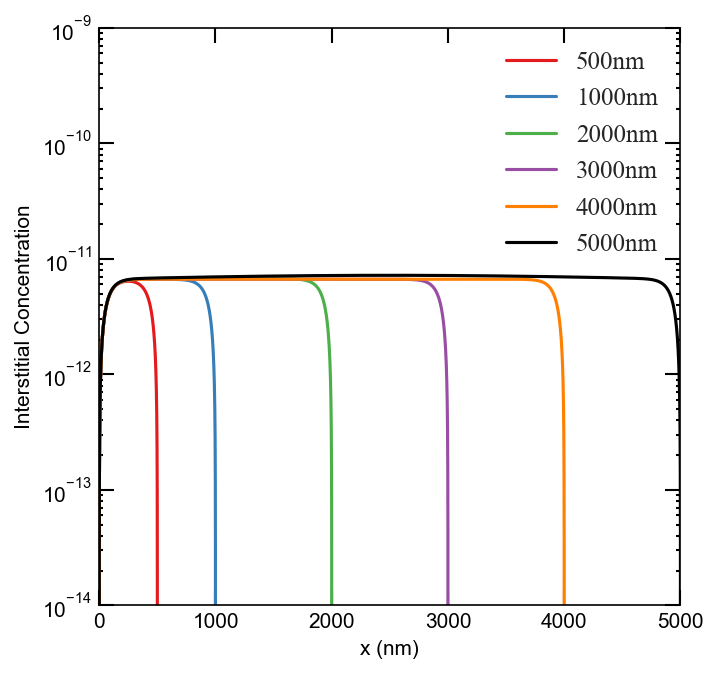
\includegraphics[scale=0.6]{interstitial_concentration_500-5000nm-neutron-0}}
        \qquad
        \subfloat{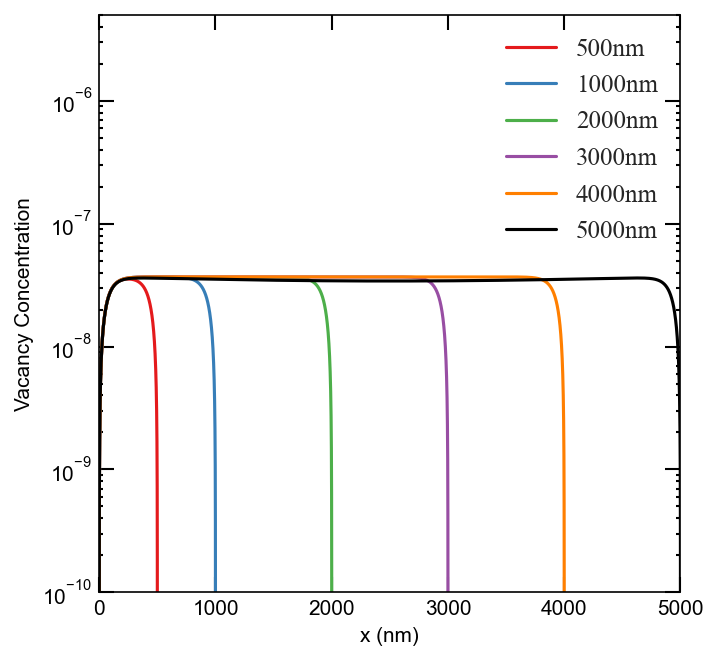
\includegraphics[scale=0.6]{vacancy_concentration_500-5000nm-neutron-0}}
        \caption{Concentration profiles for neutron irradation with 0\% Production Bias}
        \label{figure:concentrations_neutron_0_1e-6}
      \end{figure}
      \begin{figure}[h!]  %Neutron - 1e-3 dpa/s - %0 Bias rate
        \centering
        \subfloat{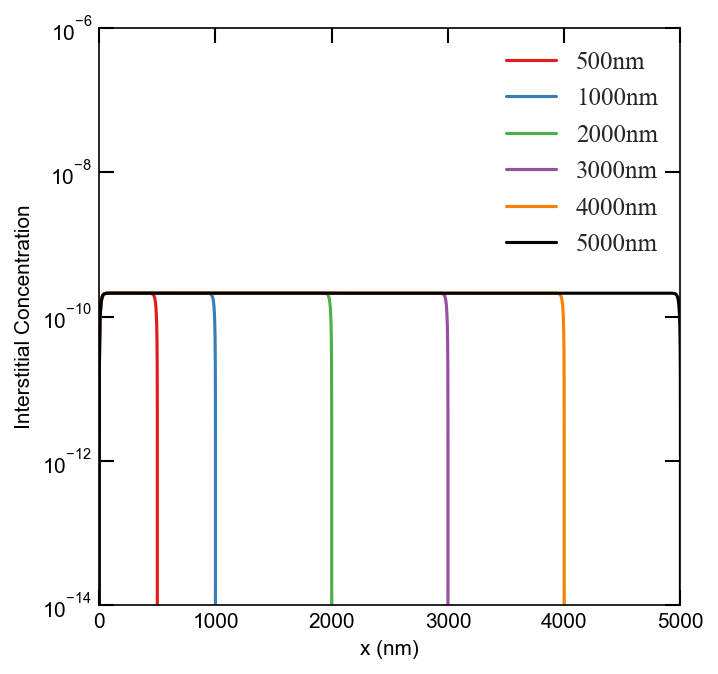
\includegraphics[scale=0.6]{interstitial_concentration_500-5000nm-high_neutron-0}}
        \qquad
        \subfloat{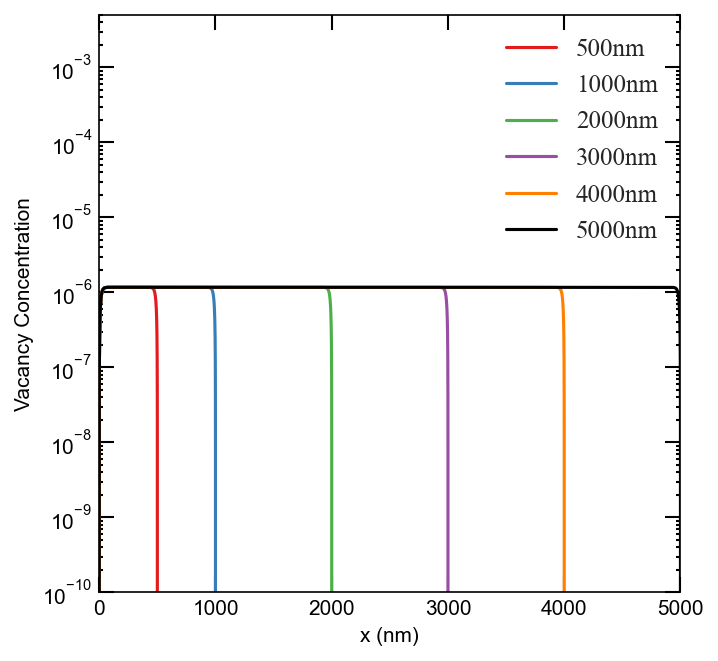
\includegraphics[scale=0.6]{vacancy_concentration_500-5000nm-high_neutron-0}}
        \caption{Concentration profiles for high dose neutron irradation with 0\% Production Bias}
        \label{figure:concentrations_neutron_0_1e-3}
      \end{figure}
      \begin{figure}[h!]  %Neutron - 1e-6 dpa/s - %5 Bias rate
        \centering
        \subfloat{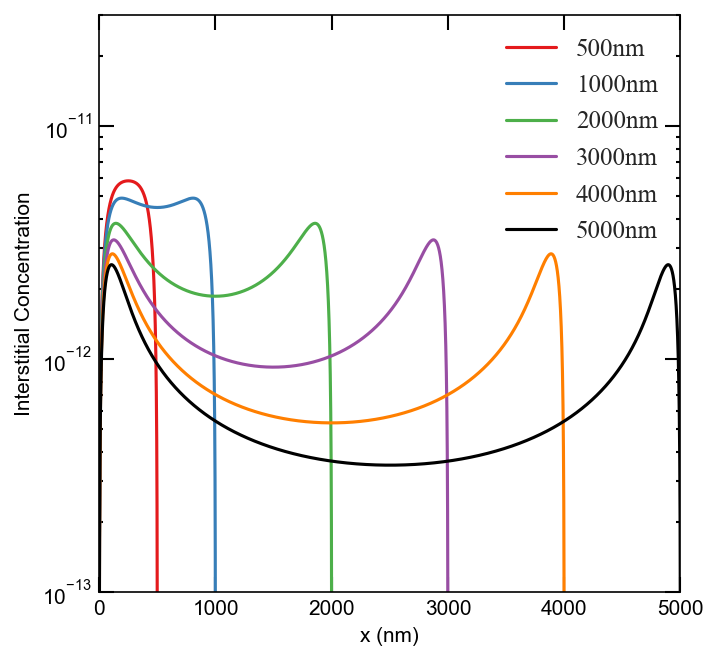
\includegraphics[scale=0.6]{interstitial_concentration_500-5000nm-neutron-5}}
        \qquad
        \subfloat{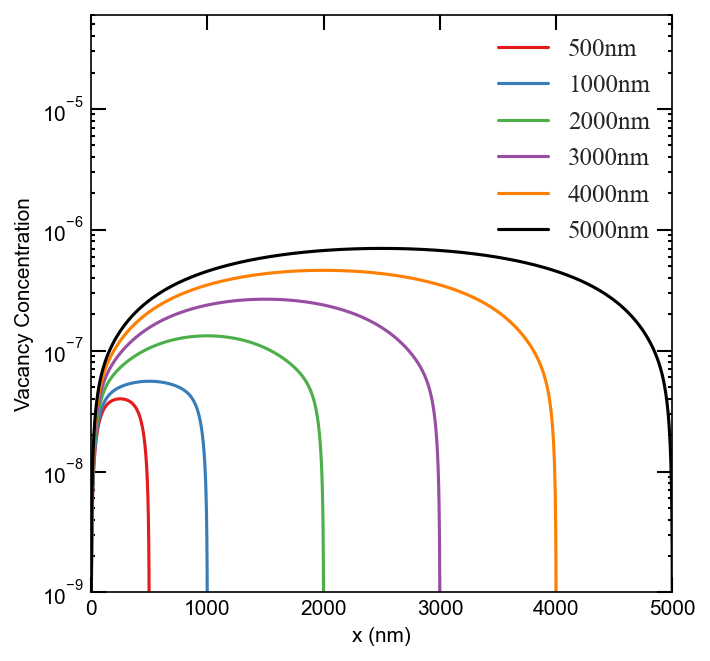
\includegraphics[scale=0.6]{vacancy_concentration_500-5000nm-neutron-5}}
        \caption{Concentration profiles for neutron irradation with 5\% Production Bias}
        \label{figure:concentrations_neutron_5_1e-6}
      \end{figure}
      \begin{figure}[h!]  %Neutron - 1e-3 dpa/s - %5 Bias rate
        \centering
        \subfloat{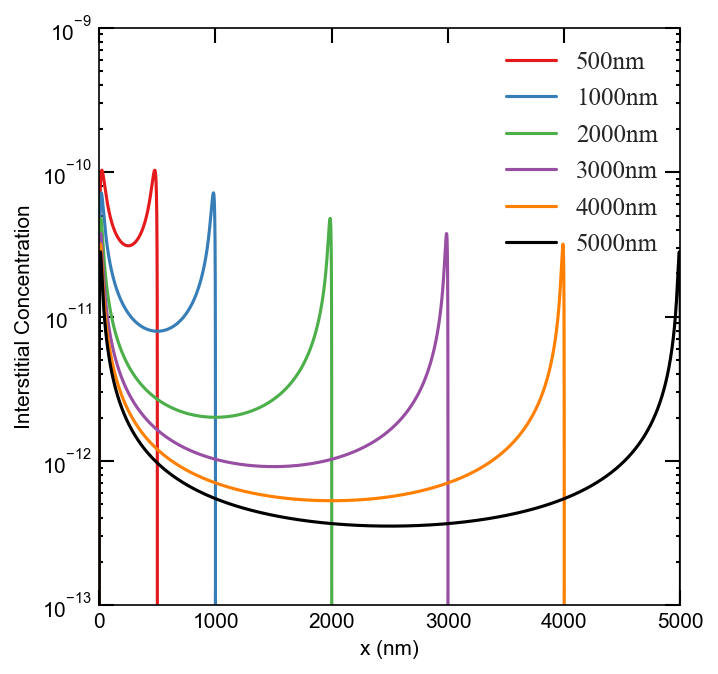
\includegraphics[scale=0.6]{interstitial_concentration_500-5000nm-high_neutron-5}}
        \qquad
        \subfloat{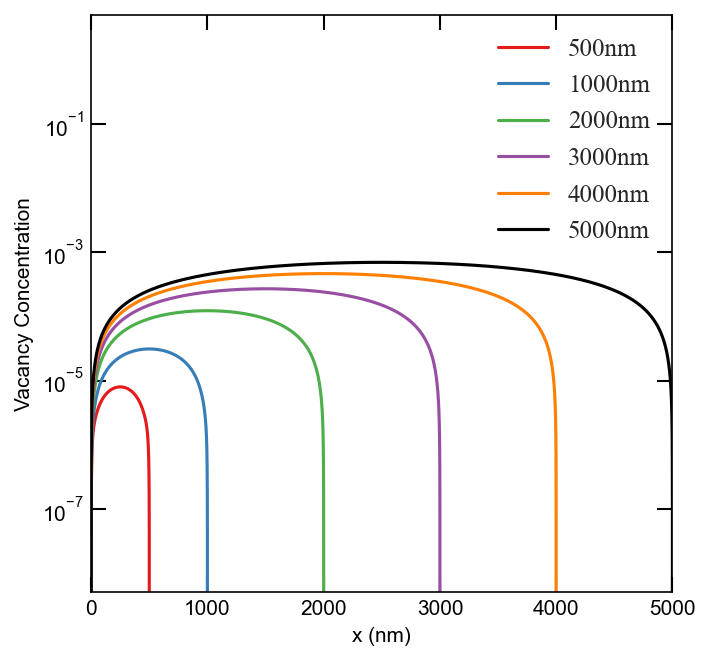
\includegraphics[scale=0.6]{vacancy_concentration_500-5000nm-high_neutron-5}}
        \caption{Concentration profiles for high dose neutron irradation with 5\% Production Bias}
        \label{figure:concentrations_neutron_5_1e-3}
      \end{figure}
      \begin{figure}[h!]  %Nuetron - Vacancy Supersaturation - 5% Bias
        \centering
        \subfloat{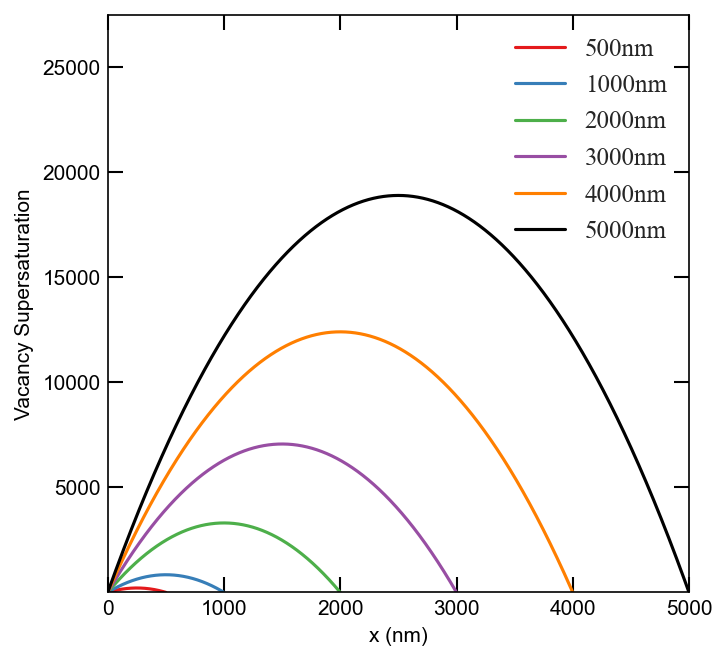
\includegraphics[scale=0.6]{super_saturation_500-5000nm-neutron-5}}
        \qquad
        \subfloat{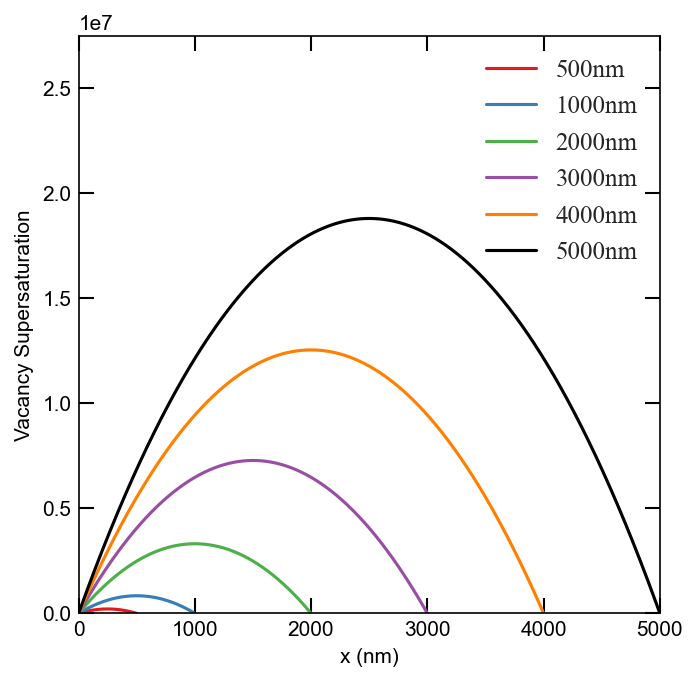
\includegraphics[scale=0.6]{super_saturation_500-5000nm-high_neutron-5}}
        \caption{Vacancy Supersaturation profiles for normal and high dose neutron irradation with 5\% Production Bias}
        \label{figure:vacancy_supersaturation_neutron_5}
      \end{figure}
    \subsubsection{Sink Strengths}
    The grain boundary sink strengths are calculated by using the equation \ref{equation:sink_strength}. First of all the defect concentration profile found by MOOSE is validated by comparing to analytical result as shown in Fig.\ref{figure:concentrations_MOOSE_analytical}
      \begin{figure}[h!]
        \centering
        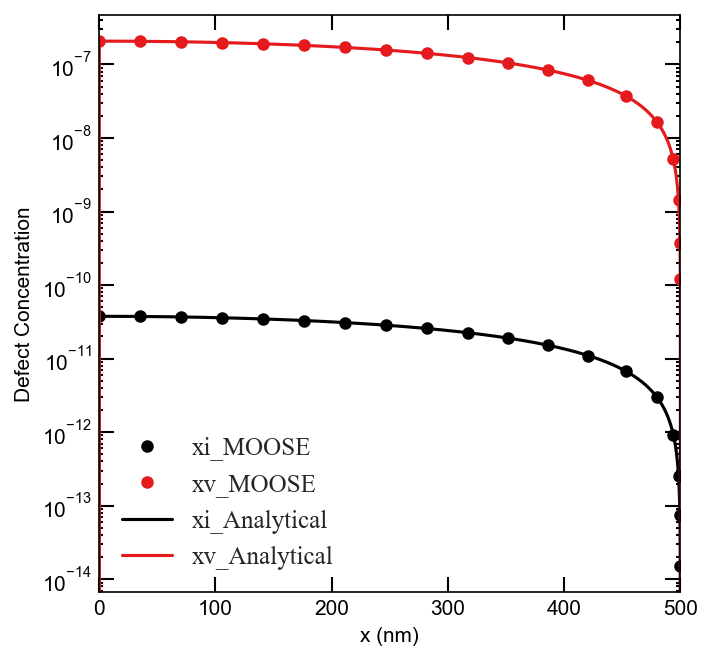
\includegraphics[scale=0.6]{concentration_profiles_MOOSE_Analytical_Neutron_0}
        \caption{Comparison of MOOSE results with analytical solution for a 1D spherical grain.\cite{heald1977}}
        \label{figure:concentrations_MOOSE_analytical}
      \end{figure}
      \begin{figure}[h!]  %Sink Strength - Neutron 1e-6 dpa/s - 0% Bias rate
        \centering
        \subfloat{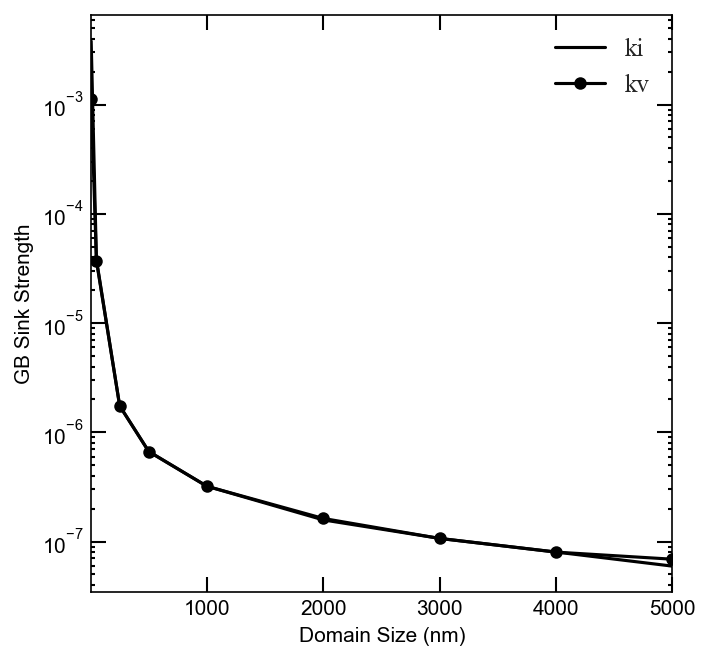
\includegraphics[scale=0.6]{sink_strength_moose_neutron_0_k}}
        \qquad
        \subfloat{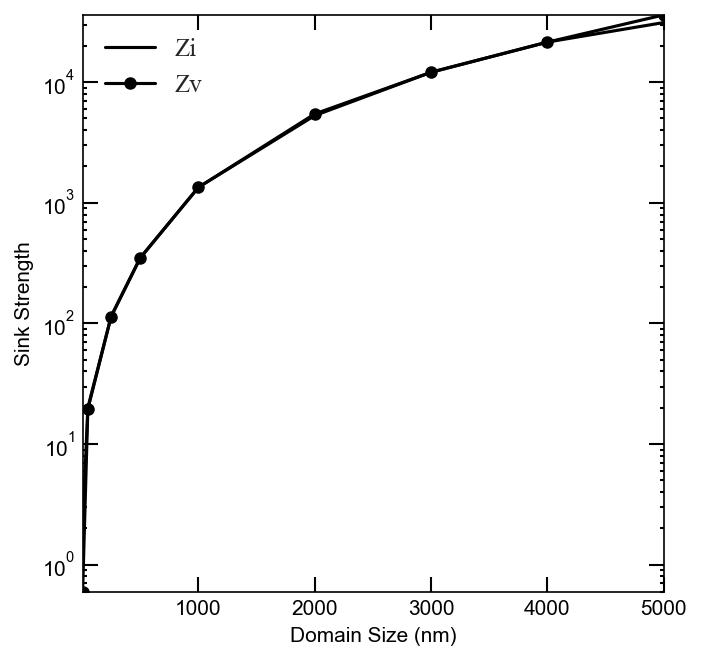
\includegraphics[scale=0.6]{sink_strength_moose_neutron_0_Z}}
        \caption{Sink Strengths for neutron irradiation with 0\% Production Bias}
        \label{figure:sink_strengths_neutron_0_1e-6}
      \end{figure}
      \begin{figure}[h!]  %Sink Strength - Neutron 1e-6 dpa/s - 5% Bias rate
        \centering
        \subfloat{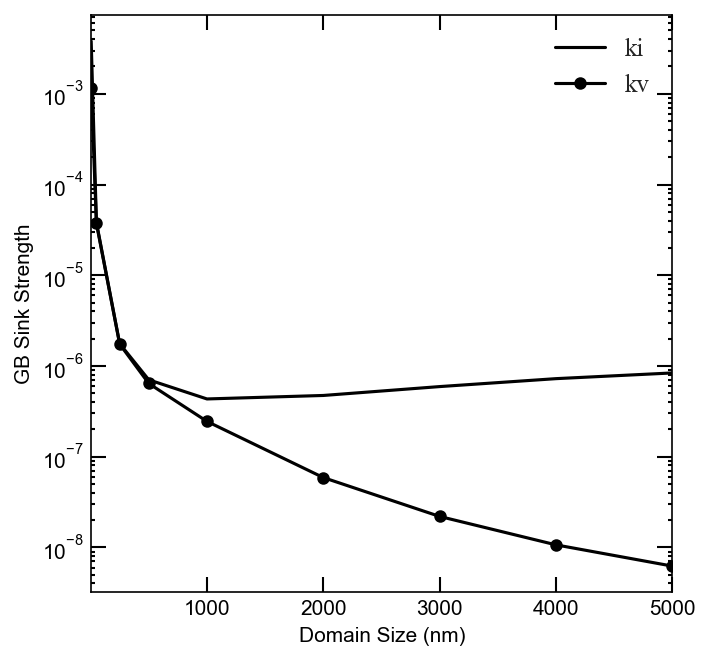
\includegraphics[scale=0.6]{sink_strength_moose_neutron_5_k}}
        \qquad
        \subfloat{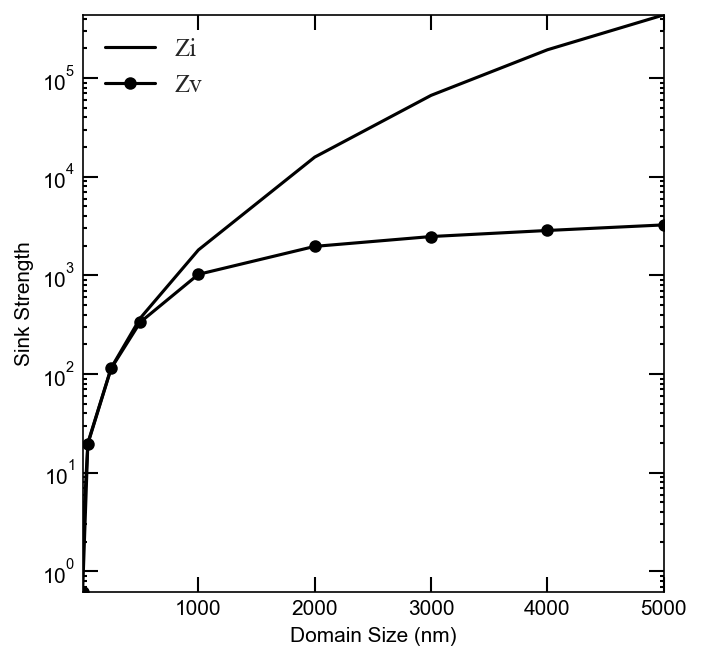
\includegraphics[scale=0.6]{sink_strength_moose_neutron_5_Z}}
        \caption{Sink Strengths for neutron irradation with 5\% Production Bias}
        \label{figure:sink_strengths_neutron_5_1e-6}
      \end{figure}

  \subsection{Ion Irradiation}
    \subsubsection{Concentrations}
      \begin{figure}[h!]  %Ion - 1e-3 dpa/s - %0 Bias rate
        \centering
        \subfloat{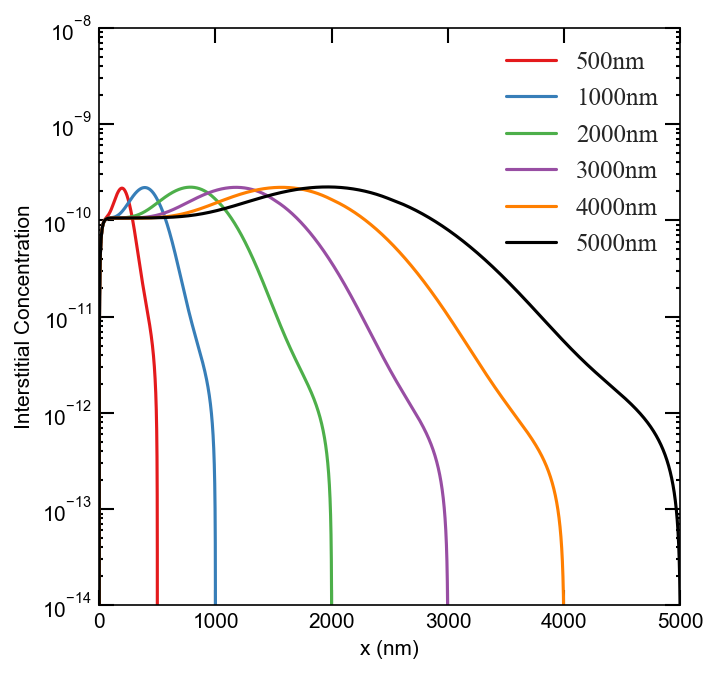
\includegraphics[scale=0.6]{interstitial_concentration_500-5000nm-ion-0}}
        \qquad
        \subfloat{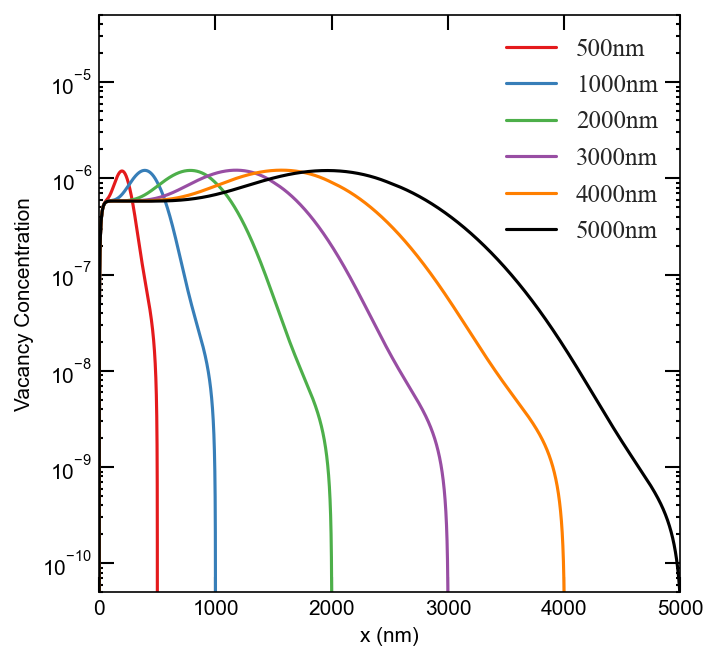
\includegraphics[scale=0.6]{vacancy_concentration_500-5000nm-ion-0}}
        \caption{Concentration profiles for low dose ion irradation with 0\% Production Bias}
        \label{figure:concentrations_ion_0_1e-6}
      \end{figure}
      \begin{figure}[h!]  %Ion - 1e-6 dpa/s - %0 Bias rate
        \centering
        \subfloat{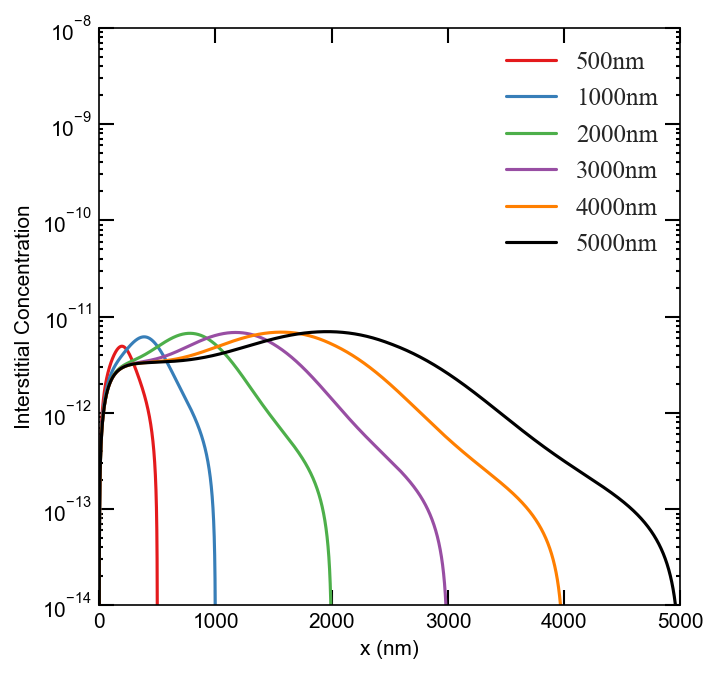
\includegraphics[scale=0.6]{interstitial_concentration_500-5000nm-low_ion-0}}
        \qquad
        \subfloat{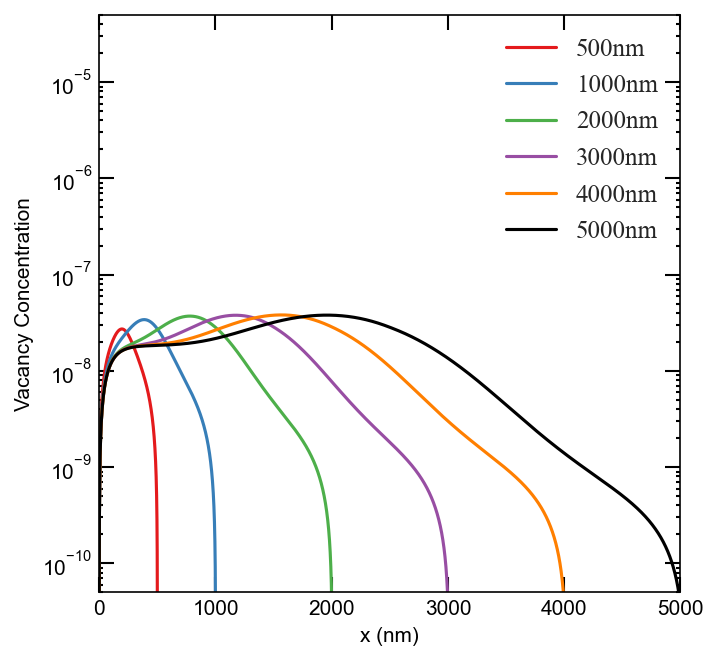
\includegraphics[scale=0.6]{vacancy_concentration_500-5000nm-low_ion-0}}
        \caption{Concentration profiles for ion irradiation with 0\% Production Bias}
        \label{figure:concentrations_ion_0_1e-3}
      \end{figure}
      \begin{figure}[h!]  %Ion - 1e-3 dpa/s - %5 Bias rate
        \centering
        \subfloat{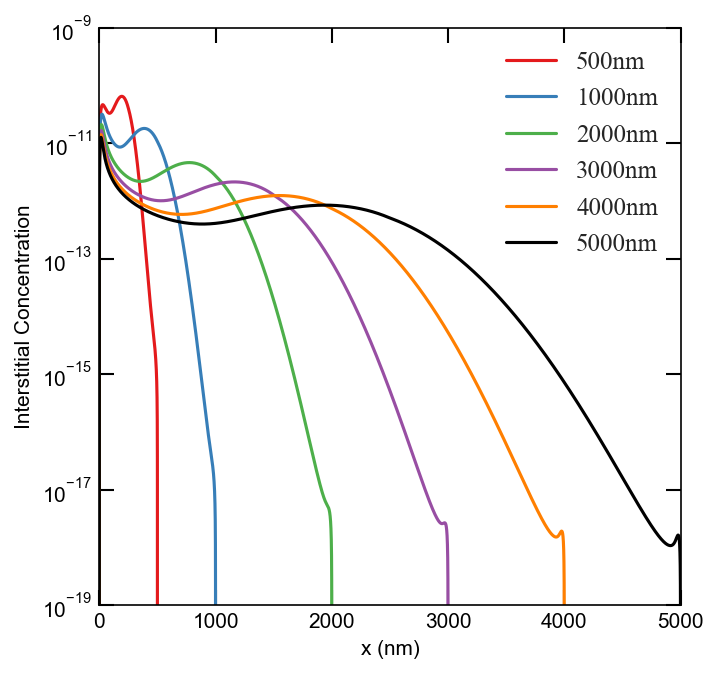
\includegraphics[scale=0.6]{interstitial_concentration_500-5000nm-ion-5}}
        \qquad
        \subfloat{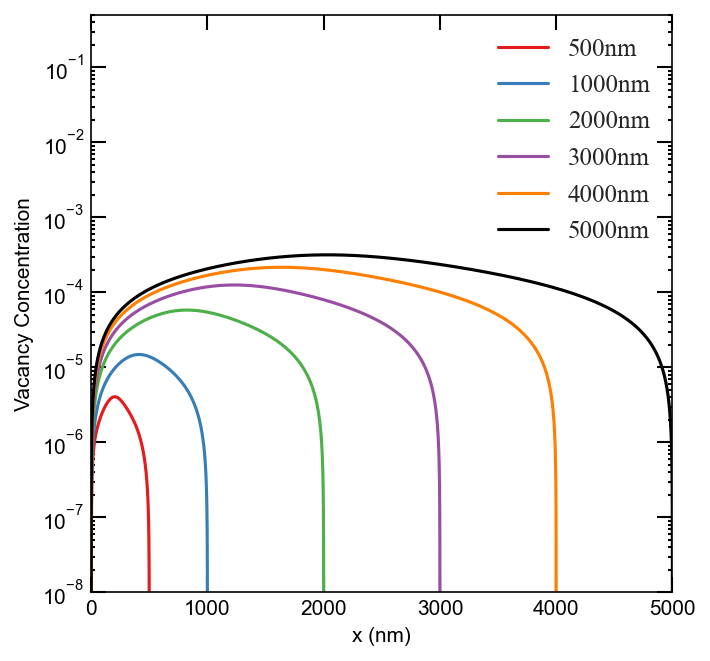
\includegraphics[scale=0.6]{vacancy_concentration_500-5000nm-ion-5}}
        \caption{Concentration profiles for low dose ion irradation with 5\% Production Bias}
        \label{figure:concentrations_ion_5_1e-6}
      \end{figure}
      \begin{figure}[h!]  %Ion - 1e-6 dpa/s - %5 Bias rate
        \centering
        \subfloat{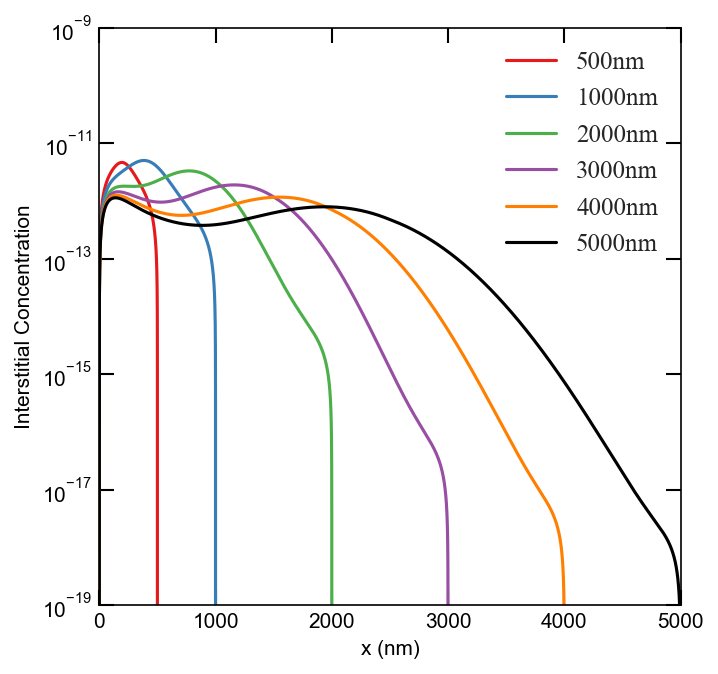
\includegraphics[scale=0.6]{interstitial_concentration_500-5000nm-low_ion-5}}
        \qquad
        \subfloat{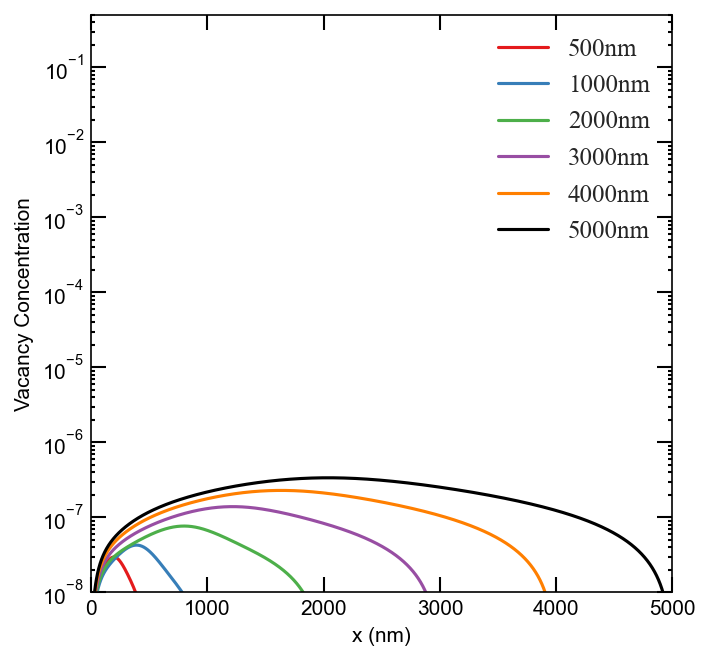
\includegraphics[scale=0.6]{vacancy_concentration_500-5000nm-low_ion-5}}
        \caption{Concentration profiles for ion irradation with 5\% Production Bias}
        \label{figure:concentrations_ion_5_1e-3}
      \end{figure}
      \begin{figure}[h!]  %Ion - %5 Bias rate
        \centering
        \subfloat{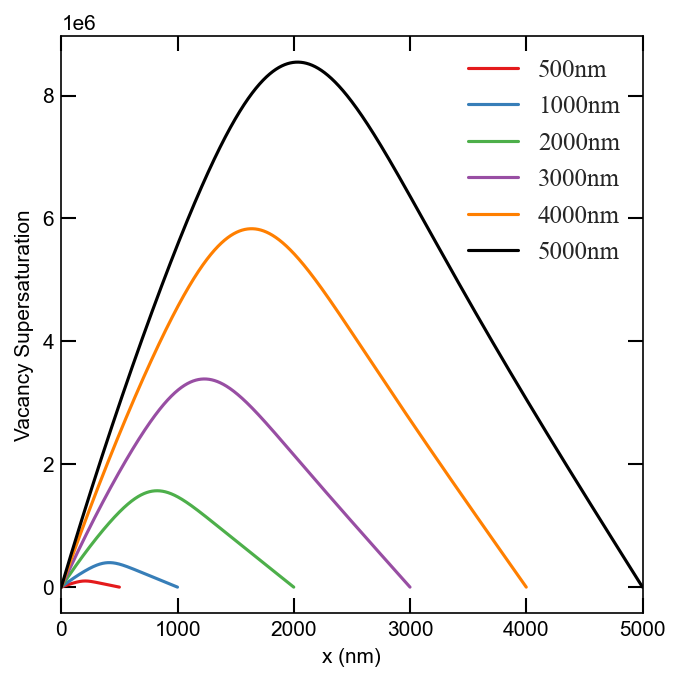
\includegraphics[scale=0.6]{super_saturation_500-5000nm-ion-5}}
        \qquad
        \subfloat{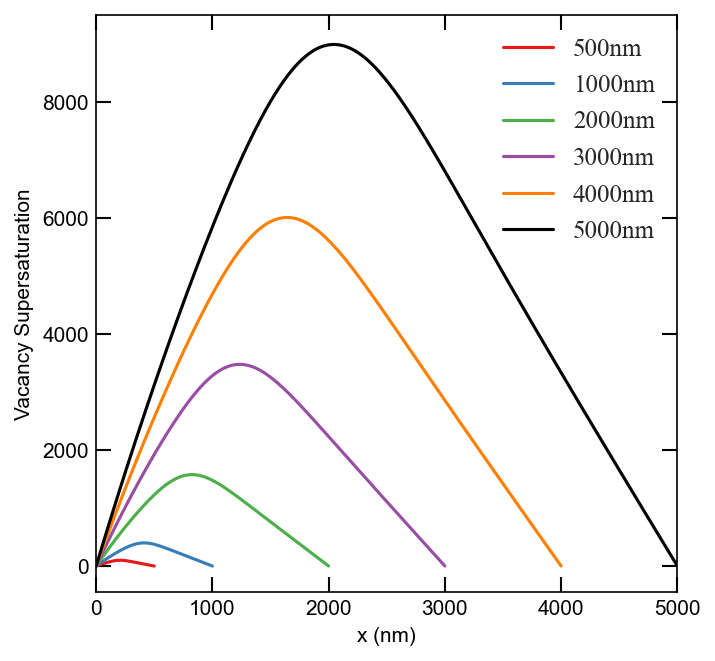
\includegraphics[scale=0.6]{super_saturation_500-5000nm-low_ion-5}}
        \caption{Vacancy Supersaturation profiles for low dose and ion irradation with 5\% Production Bias}
        \label{figure:vacancy_supersaturation_ion_5}
      \end{figure}

    \subsubsection{Sink Strengths}
      \begin{figure}[h!]  %Sink Strength - ion 1e-3 dpa/s - 0% Bias rate
        \centering
        \subfloat{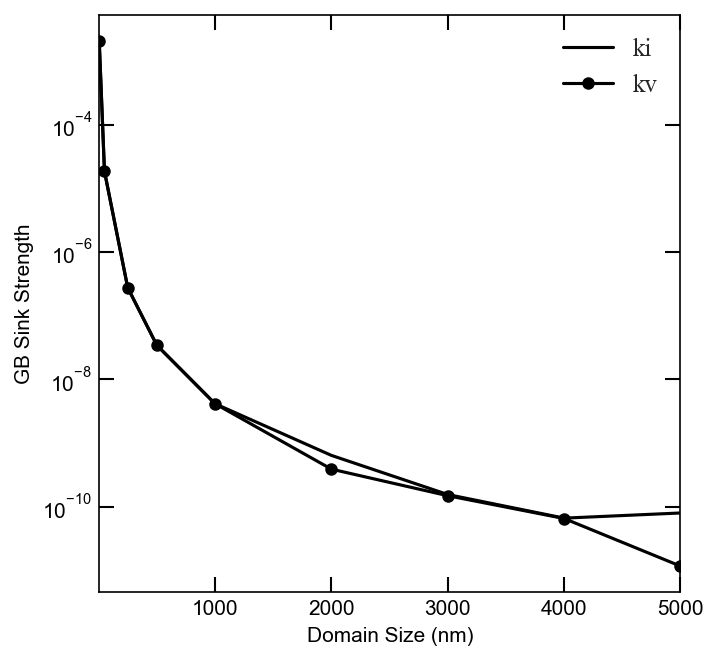
\includegraphics[scale=0.6]{sink_strength_moose_ion_0_k}}
        \qquad
        \subfloat{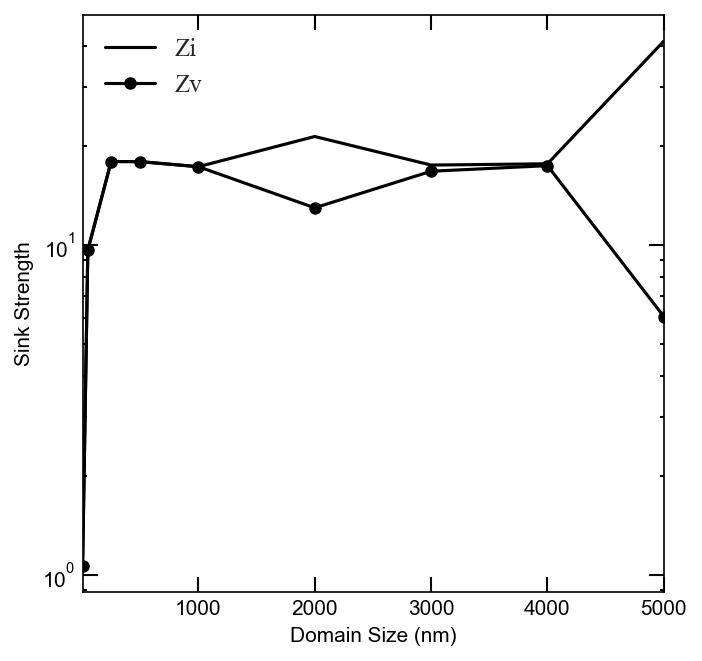
\includegraphics[scale=0.6]{sink_strength_moose_ion_0_Z}}
        \caption{Sink Strengths for low dose ion irradation with 0\% Production Bias}
        \label{figure:sink_strengths_ion_0_1e-6}
      \end{figure}
      \begin{figure}[h!]  %Sink Strength - ion 1e-3 dpa/s - 5% Bias rate
        \centering
        \subfloat{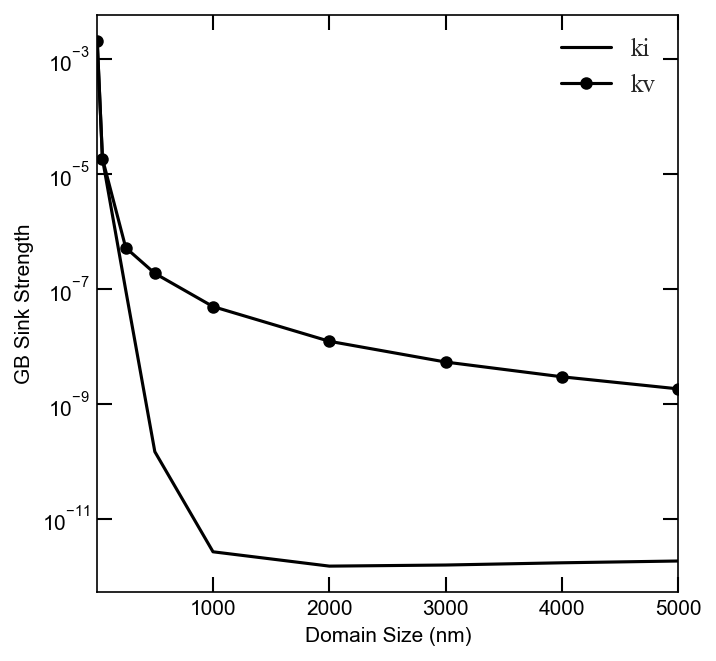
\includegraphics[scale=0.6]{sink_strength_moose_ion_5_k}}
        \qquad
        \subfloat{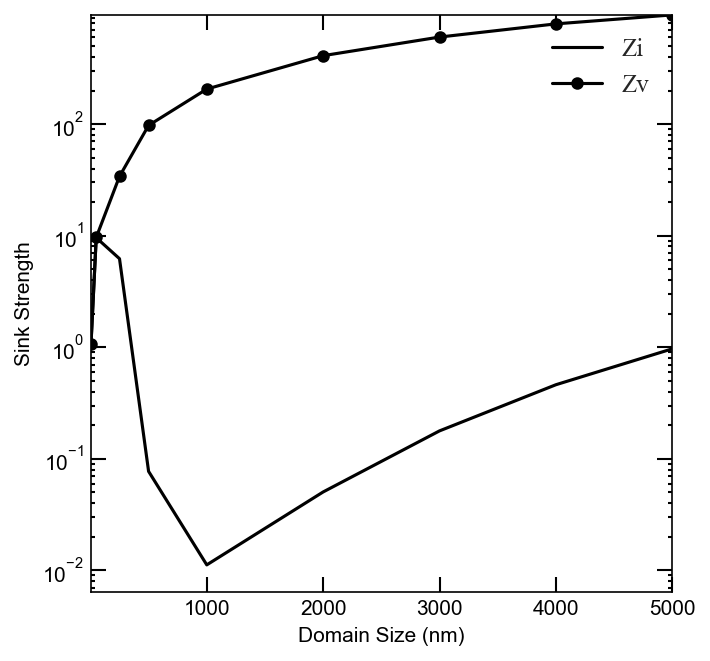
\includegraphics[scale=0.6]{sink_strength_moose_ion_5_Z}}
        \caption{Sink Strengths for ion irradiation with 5\% Production Bias}
        \label{figure:sink_strengths_ion_5_1e-6}
      \end{figure}


In nano-scale case, since the domain size is not big enough, the boundaries become
closer to each other. This causes point defects to reach sinks before they react with each other
and recombination plateau to disappear as it can be seen in Fig. 2. The nanoscale case acts like
a high-sink and high-temp condition case despite its low-sink and low-temperature. Therefore,
change in production bias does not have a significant effect on average concentration behavior
in nanoscale

On the other hand, in micro-scale case, the domain has reasonable size, and thus
boundaries are far from each other. This provides defects more time to accumulate inside the
domain and recombine with each other after they reach a specific concentration. Figure 3
clearly shows the effect of production bias on average concentration.

Effect of production bias on spatial profile of defect concentrations for nanoscale is
shown in Figure 4. The results seem not affected too much because of the same reasons
mentioned previously for average concentration.

The micro-scale results (Fig. 5) are quite interesting and worth to think over. The
concentration profiles of interstitials for 0.1%, 5% and 10% cases are flipped over. A closer look
at evolution of 5% case over time in Fig. 6, after the end of quasi-steady-state region (t=10 -4 s in
Fig 3.), the average interstitial concentration starts to decrease as they segregate through sinks.
At steady state, the average interstitial concentration becomes minimum at the center and
maximum near boundaries because of segregation.

The defect production rate (K 0 ) is the source term in point defect equations and has a
significant effect on concentrations.
In nano-scale case, the average concentration behavior is like high-sink density behavior
because of narrow domain. But, when the defect production rate increases, the average
concentration is shifted upward, and interstitial and vacancy average concentrations get closer
to each other because the production compensates more absorption at sinks than previous.
Based on this, if the production rate increased sufficiently, the recombination zone would
appear again in nano-scale domain.\cite{was2016}

\section{Conclusion} \hspace{10pt}

The most significant parameters are found as domain size and bias rate as shown in plots in this section.

% \begin{thebibliography}{00}
% \bibitem{b2} Garry S. Was.
% \end{thebibliography}
\addcontentsline{toc}{section}{References}
\bibliographystyle{unsrt}
\bibliography{ref}

\end{document}
